\section*{Introduction}
Dans ce chapitre, nous expliquerons en détail les méthodes que nous avons
employées pour l’ADT.\\
Pour commencer, nous exposerons une description de la notation de la batterie
ainsi qu’une modélisation de celle-ci pour la représentation des données
rythmiques en arbres syntaxiques. Nous poursuivrons avec une présentation de
qparse\footnote{https://qparse.gitlabpages.inria.fr/}, un outil de
transcription qui est développé à l'Inria, l'Université de Nagoya et plusieurs
développeurs au sein du laboratoire Cedric au CNAM.

Enfin, nous présenterons les forme rythmiques, <flo>une représentation
théorique qui permet…</flo> 

\section{La notation de la batterie}
\label{notation_batterie}
Pour la transcription, j’ai choisi d’utiliser une notation inspirée du recueil
de pièces pour batterie de J.-F. Juskowiak \cite{jusko} et des méthodes de
batterie Agostini \cite{ago_meth_3}, car je trouve la position des éléments
cohérente et intuitive (voir section \ref{hauteurs}).\newpage

\subsection*{Les hauteurs et les têtes de notes}
\label{hauteurs}
\begin{figure}[h]
\centering
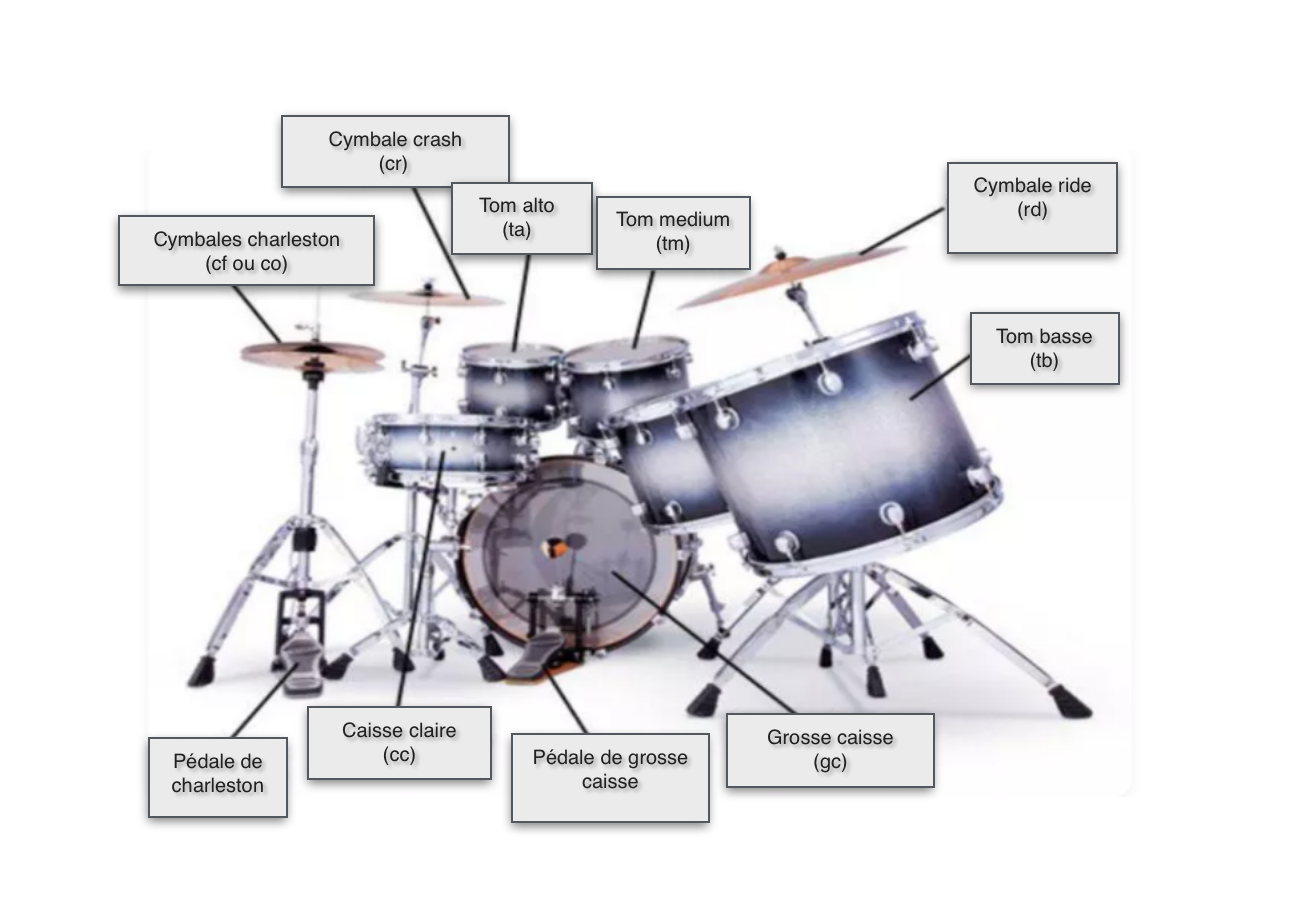
\includegraphics[height=50mm, width=80mm]{
z_images/3_methodes/0_notation_de_la_batterie/batterie.png}
\caption{Les instruments de la batterie}
\label{instru_batt}
\end{figure}

\begin{figure}[!h]
\centering
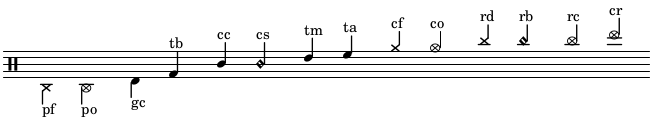
\includegraphics[height=25mm, width=130mm]{
z_images/3_methodes/0_notation_de_la_batterie/2_hauteurs_et_tete_de_notes.png}
\caption{Hauteur et têtes de notes}
\label{haut}
\end{figure}

\begin{table}[h]
\centering
\begin{tabular}{|c|c|c|} \hline
Noms figure \ref{instru_batt} & codes figure \ref{haut}  & référence \\ \hline
Pédale de charleston & pf ou po & charley fermé ou ouvert au pied \\
Grosse caisse & gc & grosse caisse \\
Tom basse & tb & tom basse \\
Caisse claire & cc & caisse claire \\
Tom médium & tm & tom médium \\
Tom alto & ta & tom alto \\
Cymbales charleston & cf ou co & charley fermé ou ouvert à la main \\
Cymbales ride & rd & ride \\
Cymbales crash & cr & crash \\ \hline
	\end{tabular}
	\caption{Noms des instruments de la batterie}
	\label{nom_instru_batt}
\end{table}
La figure \ref{instru_batt}\footnote{Source : \url{
https://www.superprof.fr/blog/composition-instrument-percussion/}} montre une
batterie standard avec tous les instruments habituellement présent sur une
batterie et la figure \ref{haut} donne leur représentation sur une partition.

Le tableau \ref{nom_instru_batt} donne dans l’ordre :
\begin{enumerate}
    \item les noms des instruments sur la figure \ref{instru_batt} ;
    \item leurs codes respectifs dans la figure \ref{haut} ;
    \item les noms que j’utiliserai dans le présent document pour y référer.
\end{enumerate}
Les figures \ref{instru_batt}, \ref{haut} et le tableau \ref{nom_instru_batt}
peuvent aider à comprendre pourquoi je trouve la notation agostinienne
cohérente et intuitive.

En effet, les hauteurs sur la portée représentent :
\begin{enumerate}
	\item La hauteur physique des instruments :\\
	La caisse claire est centrale sur la portée et sur la batterie (au niveau
    de la ceinture, elle conditionne l’écart entre les pédales et aussi la
    position de tous les instruments basiques d’une batterie).\\
	Tout ce qui en-dessous de la caisse claire sur la portée est en dessous de
    la caisse claire sur la batterie (pédales, tom basse) ;\\
	Tout ce qui est au-dessus de la caisse claire sur la portée, l’est aussi
    sur la batterie.\\
	\item La hauteur des instruments en terme de fréquences :\\
	Sauf pour le charley au pied et si l’on sépare en trois groupes
    (grosse caisse, toms et cymbales), de bas en haut, les instruments vont du
    plus grave au plus aigu.
\end{enumerate}

\subsection*{Les durées}
\label{hho}
Comme nous venons de la voir, la majorité des instruments de la batterie sont
représentés par les têtes des notes. De plus, le seul instrument dont le son
peut être arrêté de manière quantifiée et dont la durée sonore nous intéresse
est le charley\footnote{Je ne prendrais pas en compte l’arrêt des cymbales à la
main car ce phénomène n’existe pas dans les fichiers MIDI.}.
\florent{certaines têtes de notes vides alors que leur durée n'est pas celle
des blanches? expliquer les différences avec la notation conventionnelle cf
1.4}

Par conséquent :
\begin{enumerate}
    \item les durées — sauf pour le charley — représenterons un écart temporel
        entre les notes et non une durée sonore et elles pourront donc être
        rallongée à l’aide de silences ;
    \item les symboles rythmiques concernant les têtes de note ne pourront pas
        être utilisés pour exprimer les durées. Cela est valable aussi pour la
        présence ou non de la hampe puisque ce phénomène n’existe qu’avec les
        têtes de notes de type cercle-vide (opposition blanche-ronde). L’usage
        des blanches existe dans certaines partitions de batterie
        \cite{system_drums} mais cela reste dans des cas très rares. Certains
        logiciels permettent de faire des blanches avec des symboles
        spécifiques à la batterie ou aux percussions mais leur lecture reste
        peu aisée et leur utilisation pour la batterie est rarissime.\\
\end{enumerate}

En résumé :
\begin{itemize}
    \item toutes les notes ont une hampe ;
    \item une notes dont la hampe n’a pas de crochet est toujours une noire ;
    \item à part pour le charley ouvert, les durées n’expriment pas la durée
        d’un son mais une distance temporelle entre deux notes.
    \item à part pour le charley ouvert, la durée d’une note peut être
        prolongée par un silence (exemple : une noire + un soupir pour exprimer
        une blanche)\\
\end{itemize}
La durée d’une note peut être prolongée par divers symboles :
\begin{itemize}
	\item Le point : il rallonge la durée d’une note de la moitié de sa valeur.
        Dans la deuxième note de l’exemple 3 de la figure \ref{point_liaison}
        est une noire pointée, elle vaut donc la durée d’une noire + une croche
        (ou de trois croche) ;
	\item La liaison : elle rallonge la durée de la première note de la durée
        de la deuxième. La deuxième note de l’exemple 4 de la figure
        \ref{point_liaison} est une croche qui est liée à une noire, sa durée
        est donc équivalente à celle d’une croche + une noire (ou de trois
        croches) ;
    \item les silences (pas pour les ouvertures de charley).
\end{itemize}

\begin{figure}[h]
	\centering
	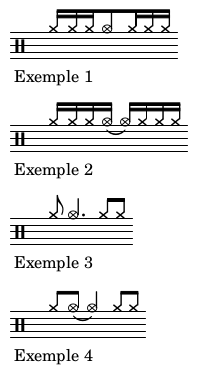
\includegraphics[height=80mm, width=40mm]{
    z_images/3_methodes/0_notation_de_la_batterie/3_point_et_liaison.png}
	\caption{Point et liaison}
	\label{point_liaison}
\end{figure}

Un autre élément concernant la notation des durées en batterie est la nécessité
de faire ressortir la pulsation\footnote{La position des temps} de la rendre
visuelle. La première chose à prendre en compte pour analyser la figure
\ref{point_liaison} est donc la nécessité de regrouper les notes par temps à
l’aide des ligatures. Le deuxième point est de s’arranger pour qu’il y ait une
indication visuelle au début de chaque temps.

\begin{itemize}
    \item Exemple 1 : l’ouverture de charley est quantifiée mais les notes ne
        sont pas regroupées par temps.
    \item Exemple 2 : Ici, la liaison permet de regrouper les notes par temps
        en obtenant le même rythme que dans l’exemple 1.
    \item Exemple 3 et exemple 4 : les deux exemples sont valables mais le
        deuxième est le plus souvent utilisé car la liaison donne un repair
        visuel sur le temps.\\
\end{itemize}

En cas de nécessité de prolonger la durée d’une note au-delà 
de son temps de départ (syncope) et si cette note ne correspond pas à une
ouverture de charley, elle sera prolongerée sur le temps suivant à l’aide de
silences dont le premier sera positionné sur le temps. Si la note syncopée est
une ouverture de charley, on privilégiera la liaison pour sa prolongation.

\subsection*{Les silences}
Les silences sont parfois utilisés pour noter les fermetures de charley (après
une ouverture). Les fermetures du charley sont notées soit par un silence
(correspondant à une fermeture de la pédale), soit par un écrasement de
l’ouverture par un autre coup de charley fermé, au pied ou à la main.

\begin{figure}[h]
	\centering
	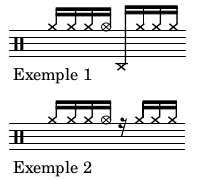
\includegraphics[height=40mm, width=40mm]{
    z_images/3_methodes/0_notation_de_la_batterie/5_silence_joue.png}
	\caption{Silence joué}
	\label{silence joue}
\end{figure}

L’écriture littérale de contenu MIDI peut ressembler à l’exemple 1 de la figure
\ref{silence joue}. Sur cet exemple, le son de l’ouverture de charley est
arrêté par une pression du pied sur la pédale et c’est ce que le batteur joue
dans les faits. Mais il apparaît intuitivement que le but de la première note
du deuxième temps n’est pas de générer un son de charley au pied mais
uniquement de stopper l’ouverture. La notation de l’exemple 2 de la figure
\ref{silence joue} serait donc préférable car elle représente mieux l’intention
de ce rythme et elle n’empiète pas sur une potentielle voix basse qui pourrait
le compléter (on évite une écriture surchargée).

Lorsqu’une note est un charley ouvert, il faudra donc prendre en compte la note
suivante pour l’écriture :
\begin{enumerate}
    \item si c’est un charley fermé joué à la main $\Rightarrow$ la note sera
        un charley fermé joué à la main (cf) ;
    \item si c’est un charley fermé joué au pied $\Rightarrow$ la note sera un
        silence.
\end{enumerate}
La deuxième règle sera soumise au cadre imposé par certaines formes rythmiques
pour lesquelles le charley joué au pied devra rester tel quel. 

\subsection*{Les équivalences rythmiques}
Pour les instruments mélodiques, dans le cas de notes dont la durée de l’une à
l’autre est ininterrompue et si leur durée initiale est prolongée, seuls la
liaison et le point permettent des notations équivalente. Mais pour la
batterie et à part dans le cas des ouvertures de charley (voir section
\ref{hho}), seules comptent des dates de début (onsets) : la durée du son n’a
pas d’importance. L’usage des silences pour combler la distance rythmique entre
deux notes devient donc possible.

Cela pris en compte, et étant donné que les indications de durée dans les têtes
de notes sont peu recommandées (voir section \ref{hho}), l’écriture à l’aide de
silences sera privilégiée comme indication de durée sauf dans les cas où cela
reste impossible. Ce choix à pour but de n’avoir qu’une manière d’écrire toutes
les notes, quelles que soient leur tête de note (sauf pour le charley).

\begin{figure}[h]
	\centering
	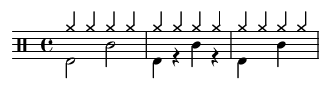
\includegraphics[height=20mm, width=75mm]{
    z_images/3_methodes/0_notation_de_la_batterie/6_equivalence.png}
	\caption{Équivalence}
	\label{equivalence}
\end{figure}

Sur la figure \ref{equivalence}, théoriquement, il faudra choisir la notation
de la deuxième mesure mais dans certains contextes, pour des raisons de
lisibilité ou de surcharge, la version sans les silences de la troisième mesure
pourra être choisie.

\subsection*{Les voix}
Pour les instruments mélodiques, un groupe de notes peut être organisé en
\emph{voix}, représentant des flots mélodiques joués en parallèle, avec une
synchronisation plus ou moins stricte \cite{SHIBATA2021262}
\cite{Guiomard-Kagan}.
% voir ref [15] ou [16] de SHIBATA….

En batterie, une voix est théoriquement l’ensemble des instruments qui, à eux
seuls, constituent une phrase rythmique. Mais en pratique, les instruments
peuvent aussi être divisés par voix dans le but de ne pas surcharger la
notation ou pour que leur disposition soit représentée sur la
partition (voir section \ref{notation_batterie}).
Les voix sont charactérisées par l’orientation des hampes et plus présicément
par les ligatures si les hampes sont dans la même direction (voir figure
\ref{afro_latin}).

\begin{figure}[h]
	\centering
	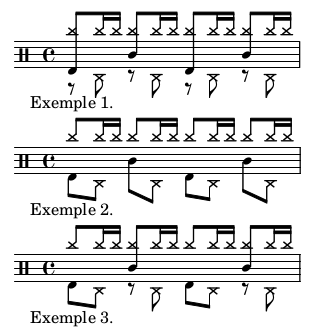
\includegraphics[height=65mm, width=60mm]{
    z_images/3_methodes/0_notation_de_la_batterie/7_voix.png}
	\caption{Séparation des voix}
	\label{sep_voix}
\end{figure}
Sur la figure \ref{sep_voix}, il faudra faire un choix entre les exemples 1, 2
et 3 qui sont trois façons équivalentes d’écrire le même rythme.
Ce choix se fera en fonction des instruments joués, de la nature plus ou moins
systèmatique de leurs phrasés, et des associations logiques entre les
instruments dans la distribution des rythmes sur la batterie (voir la section
\ref{sys_sep_voix}).

\subsection*{Les accentuations et les ghost-notes}
« Certaines notes dans une phrase musicale doivent, ainsi que les différentes
syllabes d’un mot, être accentuées avec plus ou moins de force, porter une
inflexion particulière. » \cite{danhauser}
\begin{figure}[h]
\centering
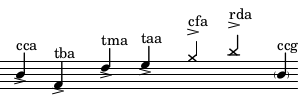
\includegraphics[height=25mm, width=75mm]{
z_images/3_methodes/0_notation_de_la_batterie/8_accents_et_ghost-notes_0.png}
\caption{Les accents et les ghost-notes}
\label{accents_et_gn}
\end{figure}

La figure \ref{accents_et_gn} ne prend en compte que les accents 
\florent{3.9 = liste des seuls "instruments" qui peuvent être accentués?}
que j’ai estimés nécessaires (voir la section \ref{velocite}). 
Les accents sont marqués par le symbole~«~>~». 
Il est positionné au-dessus des notes représentant des cymbales et en-dessous
des notes représentant des toms ou la caisse claire. Ce choix a été fait pour
la partition de la figure \ref{partition_ref} car elle est plus lisible ainsi,
mais ces choix devront être adaptés en fonction des différents forme rythmiques reconnus (voir la section \ref{systemes_methodes}). Par exemple, pour les forme rythmiques jazz, les ligatures pour les toms et la caisse claire seront dirigés vers le bas, il faudra donc mettre les symboles d’accentuation correspondants au-dessus des têtes de notes.

La dernière note de la figure \ref{accents_et_gn} montre un exemple de ghost-notes. 
\florent{expliquer ce qu'est une \emph{ghost-notes}}
Le parenthésage a été choisi car il peut être utilisé sur n’importe quelle note sans changer la tête de note.

Pour les codes, 
\florent{les codes de notes n'ont pas encore été présentés...}
on prend le code de la note et on ajoute un « a » pour un accent et un « g » pour une ghost-note. Toutes les notes de la figure \ref{accents_et_gn} sont exposées en situation réelle dans la figure \ref{exemple_acc_et_gn}. 
\begin{figure}[h]
	\centering
	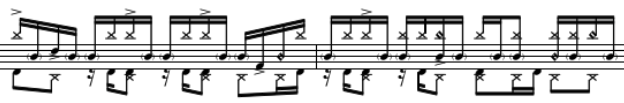
\includegraphics[height=20mm, width=110mm]{z_images/3_methodes/0_notation_de_la_batterie/8_accents_et_ghost-notes_1.png}
	\caption{Exemple pour les accentuations et les ghost-notes}
	\label{exemple_acc_et_gn}
\end{figure}
\subsection*{Les flas}
ICI, DESCRIPTION DES FLAS !
\section{Modélisation pour la transcription}
\label{modelisation_transcription}
\subsection*{Les pitchs}
\begin{table}[h]
	\centering
	\begin{tabular}{|c|c|c|} \hline
		Codes & Instruments & Pitchs \\ \hline
		cf & charley-main-fermé & 22, 42 \\
		co & charley-main-ouvert & 26 \\
		pf & charley-pied-fermé & 44 \\
		rd & ride & 51 \\
		rb & ride-cloche (bell) & 53 \\
		rc & ride-crash & 59 \\
		cr & crash & 55 \\
		cc & caisse claire & 38, 40 \\
		cs & cross-stick & 37 \\
		ta & tom-alto & 48, 50 \\
		tm & tom-medium & 45, 47 \\
		tb & tom-basse & 43, 58 \\
		gc & grosse caisse & 36 \\ \hline
	\end{tabular}
	\caption{Pitchs et instruments}
	\label{pitchs_instru}
\end{table}

Il existe, pour de nombreux instruments de la batterie, plusieurs samples audio associés à des pitchs. 
\florent{je ne comprend pas cette phrase.}
\florent{il s'agit juste d'une convention de codage des instruments de la batterie en événements MIDI...
que l'on prend en entrée pour la transcription}
Pour cette première version, nous avons choisi de n’avoir qu’un code-instrument pour différentes variantes d’un instrument, c’est pourquoi certain code-instrument se voit attribuer plusieurs pitchs dans le tableau \ref{pitchs_instru}.

Malgré le large panel de pitchs disponible, il semblerait qu’aucun pitch ne désigne le charley ouvert joué au pied. Pourtant, dans la batterie moderne, plusieurs rythmes ne peuvent fournir le son du charley ouvert qu’avec le pied car les mains ne sont pas disponibles pour le jouer. Cela doit en partie être dû à l’utilisation des boîte à rythmes en MAO qui ne nécessitent pas de faire des choix conditionnés par les limitations humaines (2 pieds, 2 mains, et beaucoup plus d’instruments…)


\subsection*{La vélocité} \label{velocite}
%\florent{j'aurais fait une section à part sur la transcription manuelle, }
La partition de la figure \ref{partition_ref} a été transcrite manuellement avec lilypond 
\florent{citation lilypond}
par analyse des fichiers MIDI et audio correspondants.

Cette transcription 
\florent{et l'analyse d'autre fichiers MIDI?}
nous a mené aux observations suivantes :
\begin{itemize}
	\item Vélocité inférieure à 40 : ghost-note ;
	\item Vélocité supérieure à 90 : accent ;
	\item Pas d’intention d’accent ni de ghost-note pour une vélocité entre 40 et 89 ;
	\item Les accents et les ghosts-notes ne sont significatifs ni pour les instruments joués au pied, ni pour les cymbales crash.\\
	En effet, certaines vélocités en dessous de 40 étant détectées et inscrites dans les données MIDI sont dues au mouvement du talon du batteur qui bat la pulsation sans particulièrement jouer le charley. Ce mouvement est perçu par le capteur de la batterie électronique mais le charley n’est pas joué.
	\item Au final, nous avons relevé les ghost-notes et les accents pour la caisse claire ainsi que les accents pour les toms et les cymbales rythmiques (charley et ride).
\end{itemize}


\subsection*{Les arbres de rythmes}
Les arbres de rythmes représentent un rythme unique dont les possibilités 
de notation sur une partition sont théoriquement multiples. 
\florent{non c'est juste une représentation du rhythme, pas unique}
\florent{expliquer le principe des RT: branchement = division d'intervalle temporel, 
feuilles = les événements musicaux commençant au début de l'intervalle).
références: 
- Laurson "Patchwork: A Visual Programming Language", 1996.
- OpenMusic: visual programming environment for music composition, analysis and research, 2011.}

Voici une représentation de la figure \ref{sep_voix} 
\florent{Fig. 3.8, ex. 1, 2 ou 3?}
en arbre de rythmes avec les codes de chaque instrument :
\begin{figure}[h]
	\Tree[ [ [rd\\gc ][ [rd\\pf ][rd ]]]
	[ [rd\\cc ][ [rd\\pf ][rd ]]]
	[ [rd\\gc ][ [rd\\pf ][rd ]]]
	[ [rd\\cc ][ [rd\\pf ][rd ]]] ]
\end{figure}

Ci-dessous, le même arbre dont les codes des instruments sont remplacés par leurs données MIDI respectives :
\begin{figure}[h]
	\Tree[ [ [51\\36 ][ [51\\44 ][51 ]]]
	[ [51\\38 ][ [51\\44 ][51 ]]]
	[ [51\\36 ][ [51\\44 ][51 ]]]
	[ [51\\38 ][ [51\\44 ][51 ]]] ]
\end{figure}

Chacun des trois exemples de la figure \ref{sep_voix} est représenté par un des deux arbres syntaxiques ci-dessus.
%\newpage


\section{Qparse}
\florent{choisir titre plus explicite, par ex. analyse syntaxique pour la transcription musicale}
La librairie Qparse\footnote{\url{https://qparse.gitlabpages.inria.fr}} 
implémente la quantification des rythmes \florent{quantification rhythmique + structuration de partition}
\florent{qparse est un outil pour la transcription musicale, qui, 
à partir d'une performance symbolique, séquentielle et non quantifiée, 
produit une partition structurée.}
\florent{Il effectue conjointement des tâches de quantification rhythmique et 
d'inférence de la structure de la partition à l'aide de technique de parsing / analyse syntaxique.}
\florent{Le but du parsing/analyse syntaxique est en effet la structuration d'une représentation séquentielle 
en entrée (un mot fini), suivant un modèle de langage.}
\florent{ref. Grune Jacobs "Parsing techniques" Springer 2007}
\florent{dans le cas de qparse, le "mot" d'entrée est typiquement au format MIDI, 
et le modèle de langage est un  un automate d'arbres pondéré représentant des préférences
en terme de notation musicale à produire.}
\florent{ref. "Handbook of weighted automata"}
basée sur des algorithmes d'analyse syntaxique pour les automates arborescents pondérés. 
En prenant en entrée une performance musicale symbolique 
(séquence de notes avec dates et durées en temps réel, typiquement un fichier MIDI), 
et une grammaire 
\florent{grammaire $\neq$ automate. il faut choisir entre les 2 (pour la suite aussi)} 
hors-contexte pondérée décrivant un langage de rythmes préférés, 
il produit une partition musicale. 
Plusieurs formats de sortie sont possibles, dont XML, MEI.

Les principaux contributeurs sont :
\begin{itemize}
	\item Florent Jacquemard (Inria) : développeur principal.
	\item Francesco Foscarin (PhD, CNAM) : \florent{apprentissage} construction de grammaire automatique 
	à partir de corpus ; Evaluation.
	\item Clement Poncelet (Salzburg U.) : integration de la librairie Midifile pour les input MIDI.
	\item Philippe Rigaux (CNAM) : production de partition au format MEI et de modèle intermédiaire de partition en sortie.
	\item Masahiko Sakai (Nagoya U.) : mesure de la distance input/output pour la quantification et CMake framework ; évaluation.
\end{itemize}

\begin{figure}[h]
	\centering
	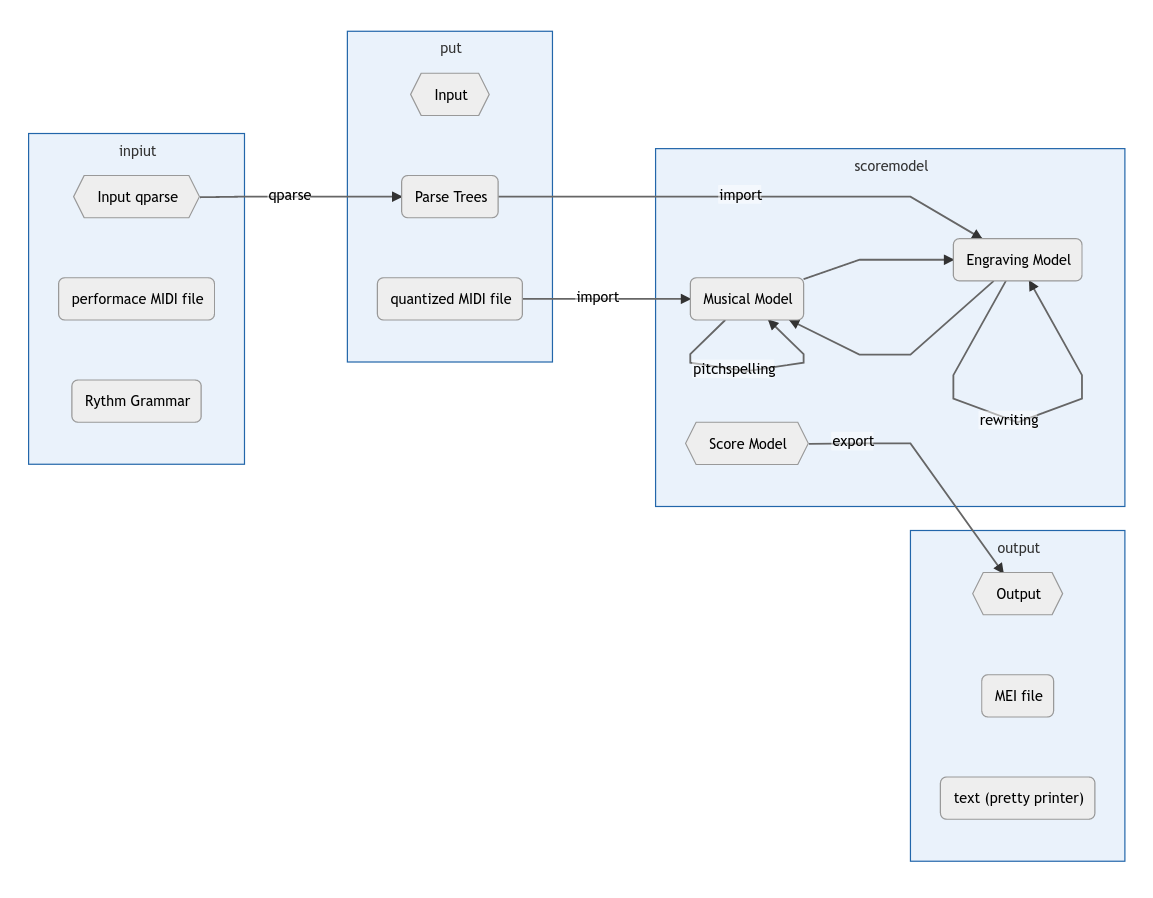
\includegraphics[height=80mm, width=130mm]{z_images/3_methodes/1_qparse/0_general_qparse.png}
	\caption{Présentation de Qparse}
	\label{presentation_qparse}
\end{figure}
\florent{la figure 3.11 est trop compliquée.
rhythm grammar $\to$ automate d'arbres pondéré.
Parse Tree $\to$ arbre syntaxique.
qtz MIDI file : inutile.
Score Model $\to$ représentation intermédiaire de partition.
Score Model, Engr. Model : inutile. garder juste la fleche Rewriting sur S.M.}

Explication des différentes étapes 
de la figure~\ref{presentation_qparse}\footnote{\url{https://gitlab.inria.fr/qparse/qparselib/-/tree/distance/src/scoremodel}} :
\begin{itemize}
	\item \textbf{Input Qparse} :\\
	Un fichier MIDI (séquence d’événements datés (piano roll) accompagné d’un fichier contenant une grammaire pondérée) ;
	\item \textbf{Arbre de parsing} :\\
	Les données MIDI sont quantifiées, les notes de dates proches sont alignées et les relations entre les notes sont identifiées (accords, fla, etc…) ; un arbre de parsing global est créé ;
	\item \textbf{Score Model} :
	\begin{itemize}
		\item Les instruments sont identifiés dans scoremodel/import/tableImporterDrum.cpp ;
		\item Réécriture 1 :\\
		séparation des voix $\Rightarrow$ un arbre par voix $\Rightarrow$ représentation intermédiaire (RI) ;
		\item Réécriture 2 :\\
		simplification de l’écriture de chaque voix dans la RI ;
	\end{itemize}
    \item \textbf{Output} :\\
    export de la partition. Plusieurs formats sont possibles (xml, mei, lilypond,… ).\\
\end{itemize}
Plusieurs enjeux :
\begin{itemize}
	\item Problème du MIDI avec Qparse :\\
	ON-OFF en entrée $\Rightarrow$ 1 seul symbole en sortie.
	\item Minimiser la distance entre le midi et la représentation en arbre.
	\item Un des problèmes de Qparse était qu’il était limité au monophonique.\\
	Quelles sont les limites du monophonique ?
	\begin{itemize}
		\item Impossibilité de traiter plusieurs voix et de reconnaître les accords.
	\end{itemize}
\end{itemize}


\section{Les forme rythmiques}
\label{systemes_methodes}
\florent{il faudrait expliquer là que le but est d'avoir des schemas types (= forme rythmique) pour calculer la séparation en voix.
       = une heuristique pour éviter d'avoir à explorer une grande combinatoire.
       et que, une fois le forme rythmique déterminé (ou sélectionné), la séparation se fait par réécriture du modèle
       (règles de projection et simplification)}
Un forme rythmique est la combinaison d’un ou de plusieurs éléments qui jouent un rythme en boucle (motif) et d’un autre élément qui joue un texte rythmique variable mais en respectant les règles propres au forme rythmique (gamme).

\subsection*{Définitions}
\florent{je ne comprend pas bien la définition de forme rythmique : motif + gamme ou motif + gamme + texte?
la déf. des gammes n'est pas du tout claire.}
\florent{est-ce que le motif est fixe et les gammes variables? 
est-ce le motif qui détermine la signature rythmique et les voix?}

\textit{\textbf{forme rythmique :}} motif + gamme/texte\\
\textit{\textbf{Motif :}} rythmes coordonnés joués avec 2 ou 3 membres en boucle (répartis sur 1 ou 2 voix)\\
\textit{\textbf{Texte :}} rythme irrégulier joué avec un seul membre sur le motif (réparti sur 1 voix).\\
\textit{\textbf{Gamme :}} la gamme d’un forme rythmique considère l’ensemble des combinaisons que le batteur pourrait rencontrer en interprétant un texte rythmique à l’aide du forme rythmique.

Un ensemble de forme rythmiques comprenant leur signature rythmique et leurs règles spécifiques de réécriture sera nécessaire. 
\florent{signature rythmique n'est pas défini. règles de réécriture non plus}
Les forme rythmiques devront être distribués dans 4 grandes catégories :
\begin{table}[h]
	\centering
	\begin{tabular}{|c|c|c|c|c|} \hline
		forme rythmiques & signature rythmiques & Subdivisions & Possibles & nb voix \\ \hline
		binaires & simple & doubles-croches & triolets, sextolets & 2 \\
		jazz & simple & triolets & croches et doubles-croches & 2 \\
		ternaires & complexe & croches & duolets, quartelets & 2 \\
		afros-cubains & simple & croches & - & 3 \\ \hline
	\end{tabular}
	\caption{Sytèmes}
\end{table}\\
Nous exposerons 3 forme rythmiques afin d’illustrer les propos de cette section :
\begin{itemize}
	\item 4/4 binaire 
	\item 4/4 jazz
	\item 4/4 afro-cubain
\end{itemize}
\subsection*{Objectif des forme rythmiques}
Les forme rythmiques devront être matchés sur l’input MIDI afin de :
\begin{itemize}
	\item définir une signature rythmique ;
	\item choisir une grammaire appropriée ;
	\item fournir les règles de réécriture (séparation des voix et simplification.\\
\end{itemize}

\florent{bien. il faudrait expliquer ça avant.}
La partie \textit{motif} des forme rythmiques sera utilisée pour la \textbf{définition des signature rythmiques}. 
Le \textit{motif} et la gammes des forme rythmiques seront utilisés pour la \textbf{séparation des voix}. 
Les règles de \textbf{simplification} (les combinaisons de réécritures) seront extraites des voix séparées des forme rythmiques.
\florent{pas exactement. les règles de projection et simplification font la séparation en voix: 
à partir d'un arbre syntaxique comme celui de 3.2, elles extraient 2 arbres, chacun contenant les 
évenements d'une seule voix}

\subsubsection{Détection d’indication de mesure}
La détection de la signature rythmique est importante, 
non seulement pour connaître le nombre de temps par mesure ainsi que le nombre
de subdivisions pour chacun de ces temps, mais aussi pour savoir comment écrire
l’unité de temps et ses subdivisions.

\begin{figure}[h]
	\centering
	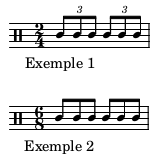
\includegraphics[height=40mm, width=40mm]{z_images/3_methodes/2_systemes/0_simple_VS_complexe.png}
	\caption{signature rythmique}
	\label{subdivisions}
\end{figure} %\newpage

La figure \ref{subdivisions} montre deux indications de mesure différentes. 
L’une (exemple 1) est \textit{simple} (2 temps binaires sur lesquels sont joués des triolets), 
l’autre (exemple 2) est \textit{complexe} (2 temps ternaires). 
Le jazz est traditionnellement écrit en binaire avec ou sans triolet (même si cette musique est dite ternaire alors que le rock ternaire sera plutôt écrit comme dans l’exemple 2).

\subsubsection{Choix d’une grammaire}
Il faut prendre en compte l’existence potentielle de plusieurs grammaires dédiées chacune à un type de contenu MIDI. 
\florent{le lien entre grammaire et signature rythmique n'est pas clair ici. 
Il aurait fallu expliquer le rôle des grammaires (automates) en 3.3}
Le choix d’une grammaire pondérée doit être fait avant le parsing puisque Qparse prend en entrée un fichier MIDI et un fichier wta (grammaire). C’est pour cette raison que la signature rythmique doit être définie avant le choix de la grammaire.

Pour les expériences effectuées avec le Groove MIDI Data Set, 
\florent{Groove MIDI Data Set pas présenté}
le style et l’indication de mesure sont récupérables par les noms des fichiers MIDI, 
\florent{méta-données}
mais il faudra par la suite les trouver automatiquement sans autres indications 
que les données \florent{contenu} MIDI elles-mêmes. 
Par conséquent, les motifs des forme rythmiques devront être recherchés sur l’input \textit{(fichiers MIDI)} 
avant le lancement du parsing, afin de déterminer la signature rythmique en amont. 
Cette tâche devra probablement être effectuée en Machine Learning. %\newpage


\subsubsection{Séparation des voix}
\label{sys_sep_voix}
\begin{figure}[h]
	\centering
	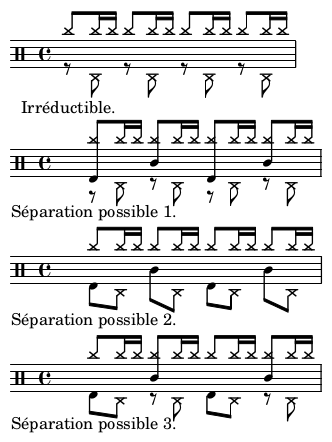
\includegraphics[height=60mm, width=40mm]{z_images/3_methodes/2_systemes/1_separation_4-4_binaire.png}
	\caption{Motif 4-4 binaire}
	\label{binaire}
\end{figure}

\florent{les description ic sont assez techniques et difficile à suivre.
avant de détailler des exemples, il faudrait décrire les objectifs et 
le principe de la procédure.}
Ici, le forme rythmique est construit sur un modèle rock en 4/4 : after-beat
sur les 2 et 4 avec un choix de répartition des cymbales type fast-jazz. La
forme rythmique est constituée par défaut du motif rd/pf/cc (voir
\ref{pitchs_instru}) et d’un gamme jouée à la grosse caisse. La première ligne
de la figure \ref{binaire} est appelée « Irréductible » car il n’y a pas
d’autre choix pertinent pour la répartition de la ride et du charley au pied.
La troisième séparation proposée est privilégiée car elle répartit selon 2
voix, une voix pour les mains (rd + cc) et une voix pour les pieds (pf + gc).
Ce choix paraît plus équilibré car deux instruments sont utilisés par voix et
plus logique pour le lecteur puisque les mains sont en haut et les pieds en
bas.
\begin{figure}[h]
\centering
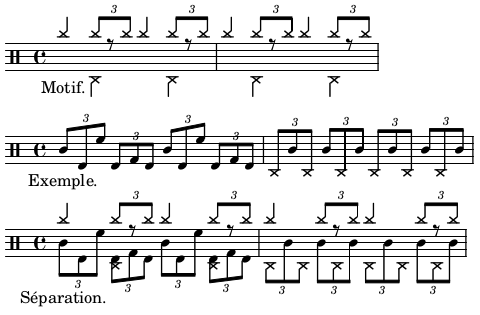
\includegraphics[height=45mm, width=60mm]{
z_images/3_methodes/2_systemes/2_separation_4-4_jazz.png}
\caption{Motif 4-4 jazz}
\label{jazz}
\end{figure}\\
Dans la plupart des méthodes, le charley n’est pas écrit car il est considéré comme évident en jazz traditionnel. Ce qui facilite grandement l’écriture : la ride et les crash sur la voix du haut et le reste sur la voix du bas. Ici, le parti pris est de tout écrire. 
Dans l’exemple ci-dessus, 
\florent{quel exemple?}
les mesures 1 et 2 combinées avec le \textit{motif} de la première ligne, sont des cas typiques de la batterie jazz. Tout mettre sur la voix haute serait surchargé. De plus, la grosse caisse entre très souvent dans le flot des combinaisons de toms et de caisse claire et son écriture séparée serait inutilement compliquée et peu intuitive pour le lecteur. Le choix de séparation sera donc de laisser les cymbales en haut et toms, caisse claire, grosse caisse et pédale de charley en bas.

\begin{figure}[h]
	\centering
	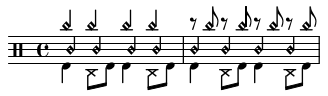
\includegraphics[height=20mm, width=70mm]{z_images/3_methodes/2_systemes/3_separation_afro-latins.png}
	\caption{forme rythmique 4-4 afro-latin}
	\label{afro_latin}
\end{figure}

La figure \ref{afro_latin} montre un exemple minimaliste de forme rythmique afro-latin \cite{system_drums}. 
Ce forme rythmique doit être écrit sur trois voix car la voix centrale est souvent plus complexe qu’ici (que des noirs) et la mélanger avec le haut ou le bas serait surchargé et peu lisible.

\subsubsection{Simplification de l’écriture}
Les explications qui suivent seront appuyé par une réécriture guidée par une
forme rythmique dans la section \ref{reecriture_guidee}.

Les gammes qui accompagnent les motifs d’un forme rythmique étayent toutes les combinaisons d’un forme rythmique et elles permettent, combinées avec le motif d’un forme rythmique, de définir les règles de simplification propres à celui-ci.

Voici les différentes étapes à suivre :
\begin{itemize}
	\item Pour chaque gamme du forme rythmique, faire un arbre de rythme représentant la gamme combinée avec le motif du forme rythmique ;
	\item Pour chaque arbre de rythmes obtenus, séparer les voix et faire un arbre de rythme par voix ;
	\item Pour chaque voix (arbre de rythmes) obtenus, extraire tous les nœuds qui nécessitent une simplification et écrire la règle.
\end{itemize}

Certaines précisions concernant l’extraction de ces règles sont nécessaires. 
Il s’agit de précisions à propos de la durée, des silences et de la présence ou non d’ouverture de charley dans les instruments joués. 
Nous avons discuté de ces problèmes dans le chapitre \ref{methodes}.

Voici quelques règles inhérentes à la simplication de l’écriture pour la batterie :
Toutes les continuations (t) qui se trouvent en début de temps 
(figures \ref{2}, \ref{4} et \ref{5}) sont transformées en silences (r) sauf si la note précédente est un charley ouvert ?
\florent{ce sont des figures et notations du chapitre suivant!}

Même si on favorise l’usage des silences pour l’écart entre les notes n’appartenant pas au même temps, on les supprime systèmatiquement pour 2 notes au sein d’un même temps et favorise, une liaison si co, un point si pas co et nécessaire, un simple ajustement de la figure de note si suffisant.

\begin{figure}[h]
	\centering
	Arbre 1
	\resizebox{70pt}{!} {
		\Tree[.1/4 [a ][b ][c ][d ] ]
	}\\
	Arbre 2\ \ \ \ \ \ \ \ 
	\resizebox{50pt}{!} {
		\Tree[.2/4 
		[ [.a ]] 
		[ [b ][c ]] ]
	}
	\caption{Simplification}
	\label{simplification}
\end{figure}
\begin{figure}[h]
	\centering
	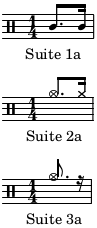
\includegraphics[height=50mm, width=20mm]{z_images/3_methodes/2_systemes/4_simplification_0.png}
	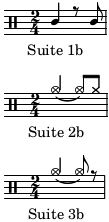
\includegraphics[height=50mm, width=20mm]{z_images/3_methodes/2_systemes/4_simplification_1.png}
	\caption{}
	\label{suites}
\end{figure}

Soit l’arbre 1 de la figure \ref{simplification} dans lequel :
\florent{itemize}
a et d sont des instruments de la batterie (x) ;\\
b et c sont des continuations (t) ;

Pour chacune des conditions suivantes, une suite de la figure \ref{suites} est attribuée :
\begin{itemize}
	\item Si a n’est pas un co :\\
	$\Rightarrow$ Suite 1a.
	\item Si a est un co :
	\begin{itemize}
		\item Si d est un cf :\\
		$\Rightarrow$ Suite 2a.
		\item Si d est un pf :\\
		$\Rightarrow$ Suite 3a : d deviens un silence (r).\\
	\end{itemize}
\end{itemize}
Soit l’arbre 2 de la figure \ref{simplification} dans lequel :\\
a et c sont des instruments de la batterie (x) ;\\
b est une continuation (t) ;
Pour chacune des conditions suivantes, une suite de la figure \ref{suites} est attribuée :
\begin{itemize}
	\item Si a n’est pas un co :\\
	$\Rightarrow$ Suite 1b, b devient un silence.
	\item Si a est un co :
	\begin{itemize}
		\item Si c est un cf :\\
		$\Rightarrow$ Suite 2b, b devient une liaison et c devient un cf.
		\item Si c est un pf :\\
		$\Rightarrow$ Suite 3b : b deviens une liaison et c devient un silence.\\
	\end{itemize}
\end{itemize}
\textit{Rappel :\\cf = charley fermé joué à la main ;\\co = charley ouvert joué à la main ;\\ pf = charley fermé joué au pied.}\\

\section*{Conclusion}
<dam>à développer un peu plus</dam>
Nous avons formalisé une notation de la batterie, modélisé cette notation pour
la transcription de données MIDI en partition, nous avons décrit Qparse.

Enfin, nous avons exposé une approche de type dictionnaire (les « forme
rythmiques ») pour détecter une signature rythmique, choisir une grammaire
pondérée appropriée et énoncer des règles de séparation des voix et de
simplification de l’écriture.
